%%%%%%%%%%%%%%%%%%%%% chapter.tex %%%%%%%%%%%%%%%%%%%%%%%%%%%%%%%%%
%
% sample chapter
%
% Use this file as a template for your own input.
%
%%%%%%%%%%%%%%%%%%%%%%%% Springer-Verlag %%%%%%%%%%%%%%%%%%%%%%%%%%
%\motto{Use the template \emph{chapter.tex} to style the various elements of your chapter content.}
\chapter{Ascent: A Flyweight In Situ Library for Exascale Simulations}
\label{ascent} % Always give a unique label
% use \chaptermark{}
% to alter or adjust the chapter heading in the running head

\abstract*{
In situ coupling poses a unique set of challenges to the design of analysis and
visualization infrastructures.
%
When running with a simulation, resources, such as time and memory are constrained.
%
As simulation applications port to accelerator-based HPC architectures, so
must our analysis tools.
%
Further, integrating into a simulation's build system adds additional complexity
becomes difficult with more dependencies.
%
Our current community tools were not designed with these set of issues in mind.
%
Ascent is an emerging is situ analysis and visualization infrastructure that
addresses these challenges.
%
From Ascent's inception, we have targeted in situ use cases and many-core
architectures.
%
In this paper, we will discuss in detail Ascent's design considerations, data and control interfaces, system architecture, and success stories.
}

This chapter describes the Ascent library for in situ visualization
and analysis.
%
Ascent was designed to deliver on two goals which are often in tension:
 (1) minimize encumbrance on simulation codes that incorporate Ascent,
i.e., a ``flyweight'' design, and
(2) deliver diverse and powerful capabilities,
especially for modern supercomputers.
%
In addition, Ascent is built for production use by computational
simulation codes --- it has documentation,
examples, engages in modern software engineering practices, etc.

In terms of flyweight design, Ascent aims to minimize
execution time, memory usage, binary size, and integration effort.
%
The first two, execution time and memory usage, benefit from directly
incorporating VTK-m~\cite{Moreland:CGA2016} into Ascent.
%
For minizing memory,
VTK-m's data model supports many array layouts (e.g., row major versus
column major, array of structures versus structures of arrays)
in a zero-copy manner.
%
In most cases, the majority of the memory needed by Ascent is only for
storing intermediate results.
%
To minimize execution time,
VTK-m provides native support for many-core architectures,
including Nvidia GPUs, various Intel architectures,
and planned support for AMD GPUs.
%
Further, Ascent complements VTK-m's shared-memory parallelism with
its own layer for distributed-memory parallelism based on the
Message Passing Interface (MPI) library.
%
In all, Ascent is able to perform its algorithms very quickly,
since it can make full use of the underlying hardware architecture.
%
\fix{Statement about binary size.}
%
Finally, Ascent's API was designed to be simple to learn,
easy to integrate for novice users, and small in overall code size.
%
Integrations can be as short as ten lines of code.
%
This topic is explored more in \S\ref{sec:API}.

In terms of delivering diverse and powerful capabilities,
Ascent employs multiple approaches:
integration with many technologies,
supporting both visualization and analysis routines,
algorithms specifically designed for in situ processing,
and providing support for modern supercomputers.
%
Ascent's strongest component for delivering capabilities is likely
through integrating many additional technologies.
%
In terms of integrations with other visualization and I/O products,
Ascent is able to produce Cinema and HDF5 files, interact with
ADIOS and Catalyst, and, as previously mentioned, utilizes VTK-m
directly for much of its data model and visualization algorithms.
%
It also provides many options for integration, including
bindings
for controlling Ascent with  C, C++, Python and Fortan.
%
Further, it provides options for controlling Ascent via its code API,
via YAML files (which can be changed dynamically at runtime), and via
a Jupyter notebook integration \fix{cite ISAV19}.
%
Finally, Ascent is able to integrate arbitrary code, including
Python scripts and C/C++ code.
%
This pathway also enables access to
machine learning infrastructures, such as TensorFlow and PyTorch.
%
This is more than proof of concept,
as Ascent recently utilized a distributed-memory Random Forest.
%
\S\ref{sec:DevilRay} describes a success story regarding integrating
code,
namely incorporating the DevilRay code for ray-tracing higher order
elements.
%
Moving to another approach, Ascent has embraced analysis alongside
visualization.
%
Noteworthy analysis examples include simulated radiographs and its
query infrastructure to get quantitative results such as volumes,
surfaces areas, and integrated quantities.
%
Of course, Ascent supports typical visualization algorithms, such as
slicing, isosurfacing, volume rendering, and multiple plot types.
%
With respect to algorithms specifically for in situ processing, Ascent
has a significant investment in its ``trigger'' system~\cite{Larsen:ISAV18},
which adapts when visualization and analysis routines are executed,
based on the conditions in the system.
%
Ascent also has algorithms for extracting reduced forms of the data,
such as a module for extracting Lagrangian flow~\cite{Agranovsky:LDAV2014,Sane:EGPGV19} and the
aforementioned Cinema output.
%
Finally, Ascent has been designed from the beginning with modern
supercomputers in mind.
%
Especially because of the integration of VTK-m, Ascent is able to
run efficiently on these architectures.

The remainder of this chapter focuses on key elements of Ascent:
\begin{itemize}
\item \S\ref{sec:capabilities} discusses the key abstractions for using Ascent.
\item \S\ref{sec:design} discusses Ascent's design.
\item \S\ref{sec:API} discusses Ascent's APIs for sharing simulation
data and for controlling execution.
\item \S\ref{sec:success} discusses success stories using Ascent.
\end{itemize}

\section{Key Abstractions for Ascent --- Matt}
\label{sec:capabilities}
This section describe Ascent's primary abstractions and surveys its general capabilities.
%
Ascent organizes its capabilities into five types of in situ tasks, which
it refers to as \textbf{actions}.
%
Its five actions are:
\begin{itemize}
\item \textbf{Pipelines} transform data from one form to another.
%
\item \textbf{Scenes} render images.
%
\item \textbf{Extracts} are used to move data out of Ascent, i.e., to file I/O or to another framework.
%
\item \textbf{Queries} provide quantitative summarizations of the data.
%
\item \textbf{Triggers} adapt when other actions are executed, based on the conditions of the simulation.
%
\end{itemize}

These actions are highly interoperable, and Ascent can employ multiple actions of the same type
at once.
%
Consider the following example of Ascent doing in situ analysis on an input data set, $D$,
for a given cycle of a simulation.
%
Ascent begins by applying an isosurfacing operation to $D$ to make a new data set $D'$ (pipeline).
%
It then applies a trigger to $D'$ --- it takes the surface area of the isosurface (query) and compares
the total area with the area from the previous time it was executed.
%
If the total area has changed by more than 5\%, then Ascent would render an image of $D'$ (scene)
and also save the original data set $D$ to disk (extract).
%
Going beyond this example, it is possible to have multiple triggers, arbitrary conditions for
the triggers (queries or otherwise), as well as many pipelines, scenes, and extracts.
%
Figure~\ref{fig:ascent_example} shows an example of this, specifically two pipelines and two extracts.

\begin{figure}
\centering
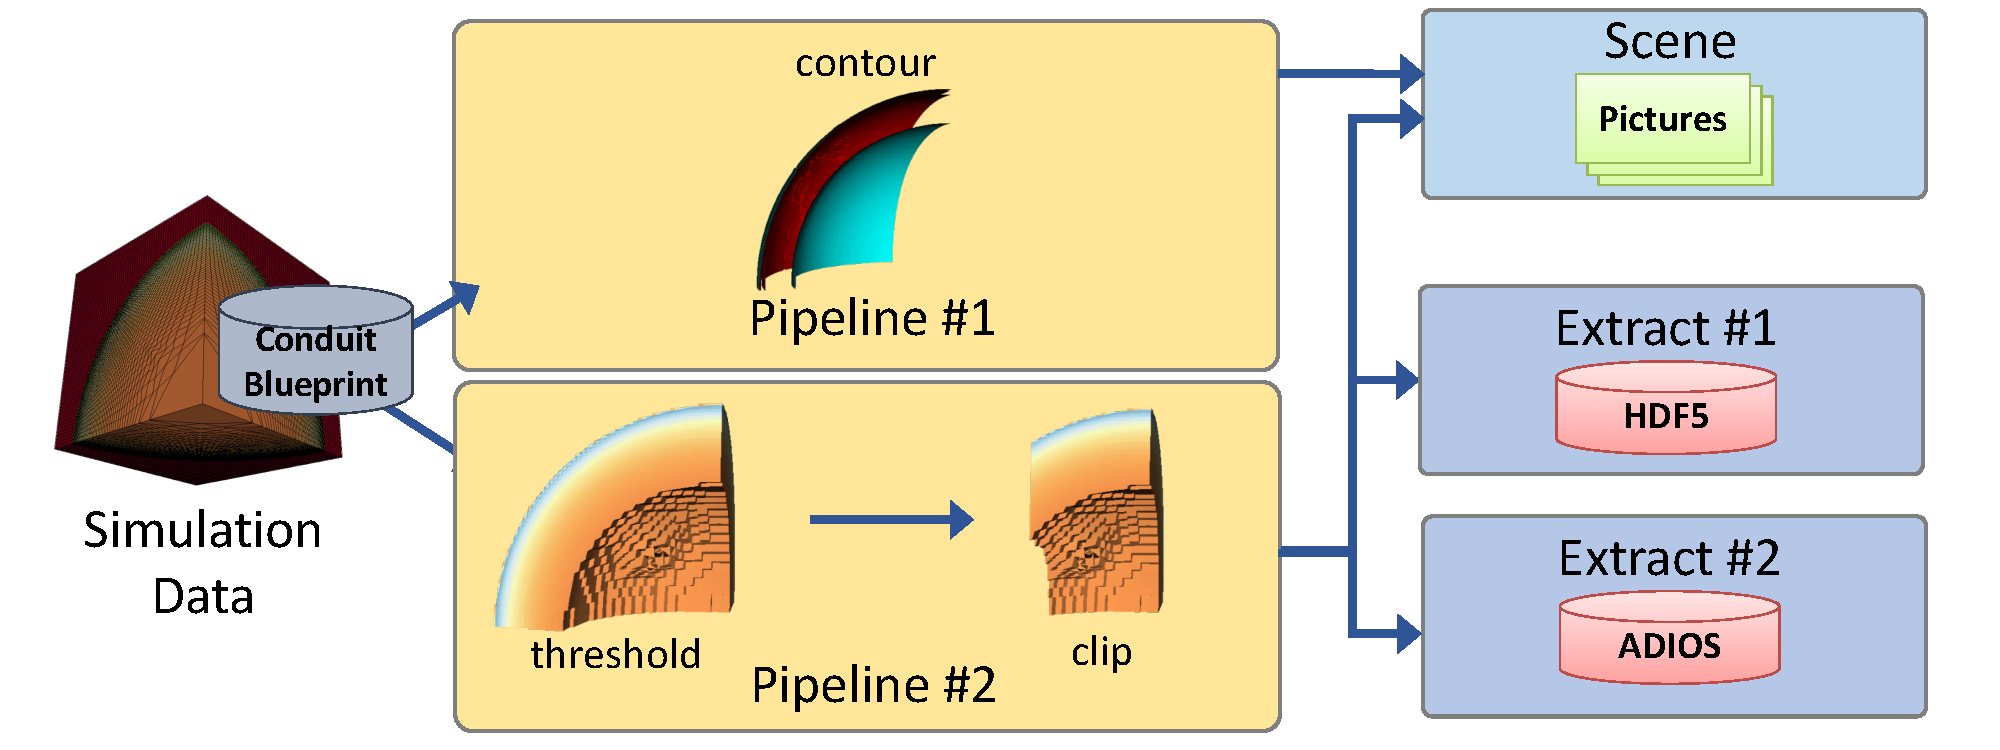
\includegraphics[width=\textwidth]{images/ascent_actions_diagram.pdf}
\caption{\label{fig:ascent_example} An example of how Ascent actions can be combined.
In this example, simulation data is acquired from Conduit/Blueprint (see \S\ref{sec:API}),
and that data is relayed into two pipelines (labeled \#1 and \#2).
The first pipeline applies a contour operation, while the second
applies threshold and clip operations.
%
The results of these pipelines are used in multiple ways.
A scene uses both pipelines as input, while two extracts use only the second pipeline
as input, outputting using two different I/O libraries.}
\end{figure}

\subsection{Pipelines}

Pipelines allows users to describe a series of data transformations, also known as filters,
to execute on simulation data.
%
%These data transformations are sometimes referred to as filters in other
%frameworks (like VTK~\cite{VTK}), and
Figure~\ref{fig:ascent_example} shows
typical filters for visualization: contour, threshold, and clip.
%Figure~\ref{img:pipelines} shows two examples of pipelines.
%%
%Pipeline \#1 creates contours from a simulation field, and pipeline \#2
%thresholds cells that are within a scalar range then applies a clipping operation.
%
Ascent allows users can define an arbitrary number of pipelines.
%
In terms of inputs and outputs, the input to a pipeline is either
the simulation data or another pipeline, and the outputs of a pipeline
can go to scenes, extracts, and queries.
%
Further, triggers can make use of pipelines, and their relationship is discussed further
in \S\ref{sec:ascent:triggers}.

%
%The default source of pipelines, and all other actions, is the data
%published by the simulation, but all actions can consume the results
%of declared pipelines, including other pipelines.

%\begin{figure}
%\centering
%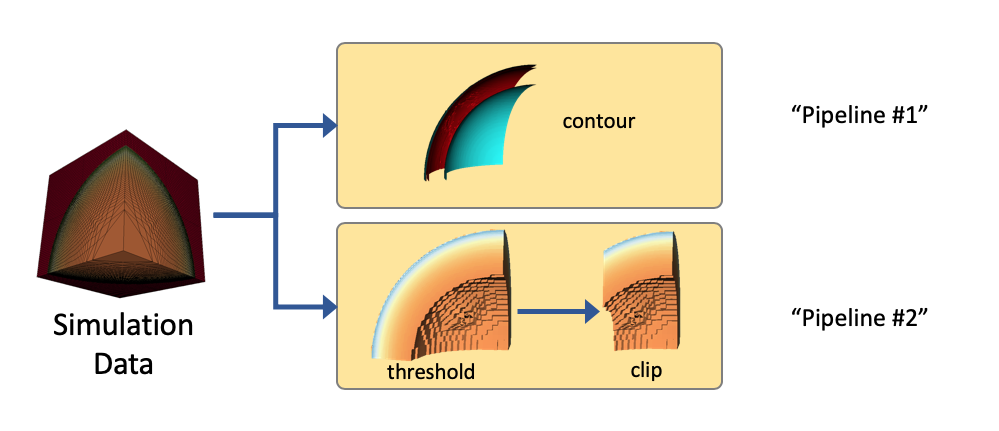
\includegraphics[width=0.6\textwidth]{images/pipelines}
%\caption{\label{img:pipelines} Examples pipelines that transforms simulation data via visualization operators.}
%\end{figure}

Notable filters currently supported by Ascent include:
\begin{multicols}{2}
\begin{itemize}
\item Clipping
\item Contour
\item Histogram
\item Isovolume
\item Particle Advection
\item Statistics
\item Slice
\item Threshold
\end{itemize}
\end{multicols}

There are also filters that create new fields: Divergence, Gradient, Logarithm, Q-Criterion, Vector Magnitude, and Vorticity.
%
Finally, Ascent contains two specific-to-in-situ filters that
reduce data size significantly enough that it can be saved to disk and explored post hoc:
Lagrangian Flow and Sampling (\fix{should be a reference here to Biswas chapter on sampling}).


\subsection{Scenes}

Scenes create images.
%
They typically operate on the output of pipelines, but they also can work directly
on the original simulation data.
%
Scenes do not return anything to Ascent that can interact with other actions, but they
do save the images they produce to disk for later inspection.

A scene is made up of ```renders''' and ```plots.'''
%
Renders can be thought of as sub-scenes, i.e., each scene is made up of many sub-scenes (renders),
which contain
camera specifications, image dimensions, background and
foreground colors, and annotation controls.
%
There can be an arbitrary number of renders for a scene. 
%
Plots are the things to render.
%
A plot consists of two things: what data to render and how to render it.
%
The data comes from the input (usually a pipeline), and the method for rendering the data can vary.
%
Currently, Ascent supports four plot types: pseudocoloring, volume rendering, mesh plots,
and radiograph plots(see Figure~\ref{fig:ascent_plots}).
%
Each of these plot types contain parameters that control the input data
(name of the pipeline to consume, which scalar field to operate on, etc.)
and how to carry out the rendering (color tables, scalar ranges, etc.).
%

\begin{figure}
\centering
  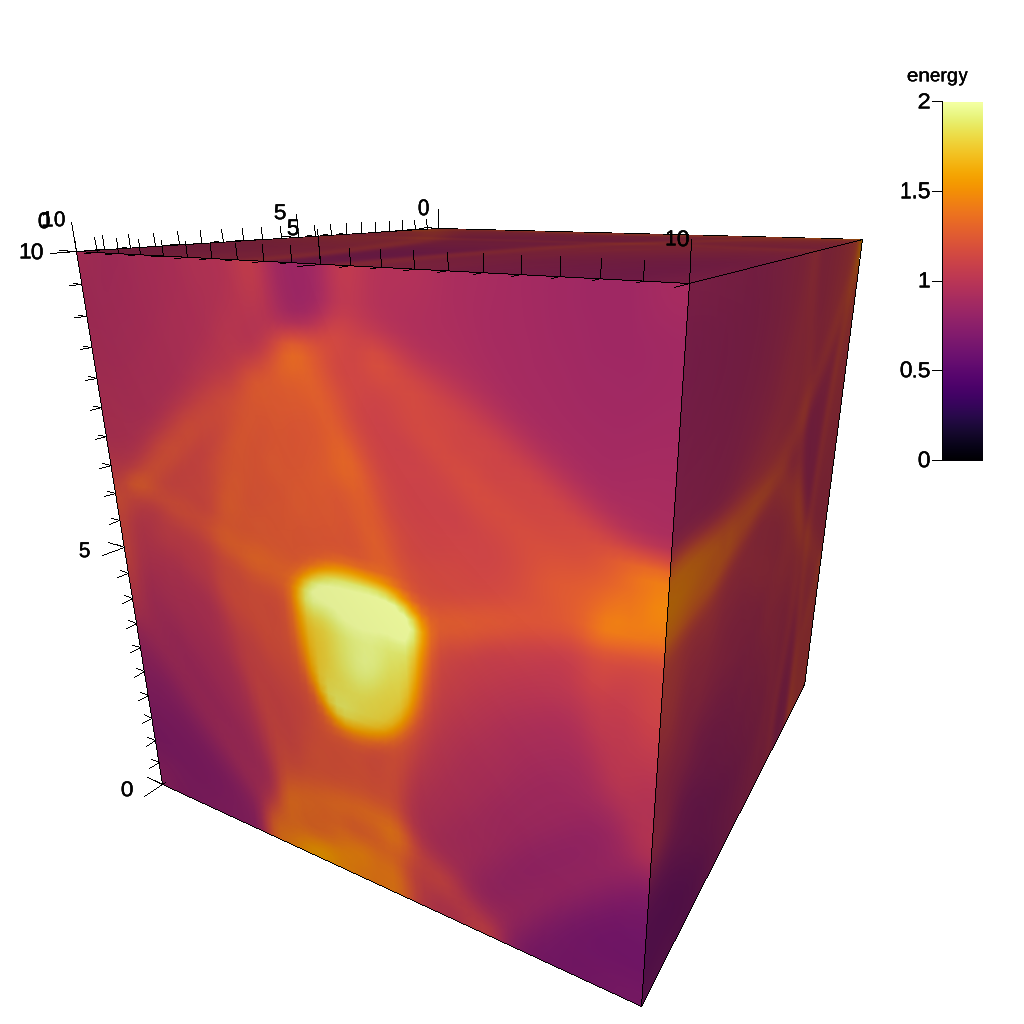
\includegraphics[width=0.4\textwidth]{images/pseudocolor250}
  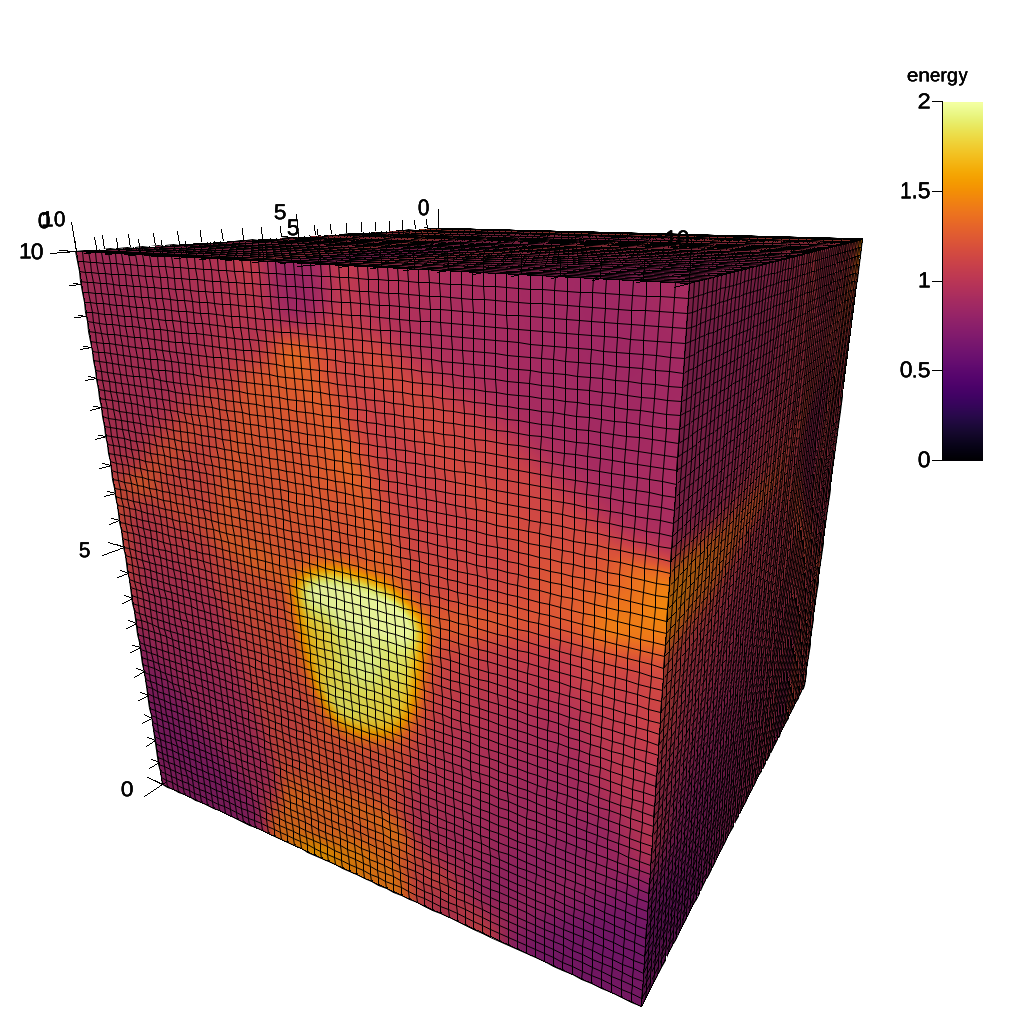
\includegraphics[width=0.4\textwidth]{images/mesh250}
  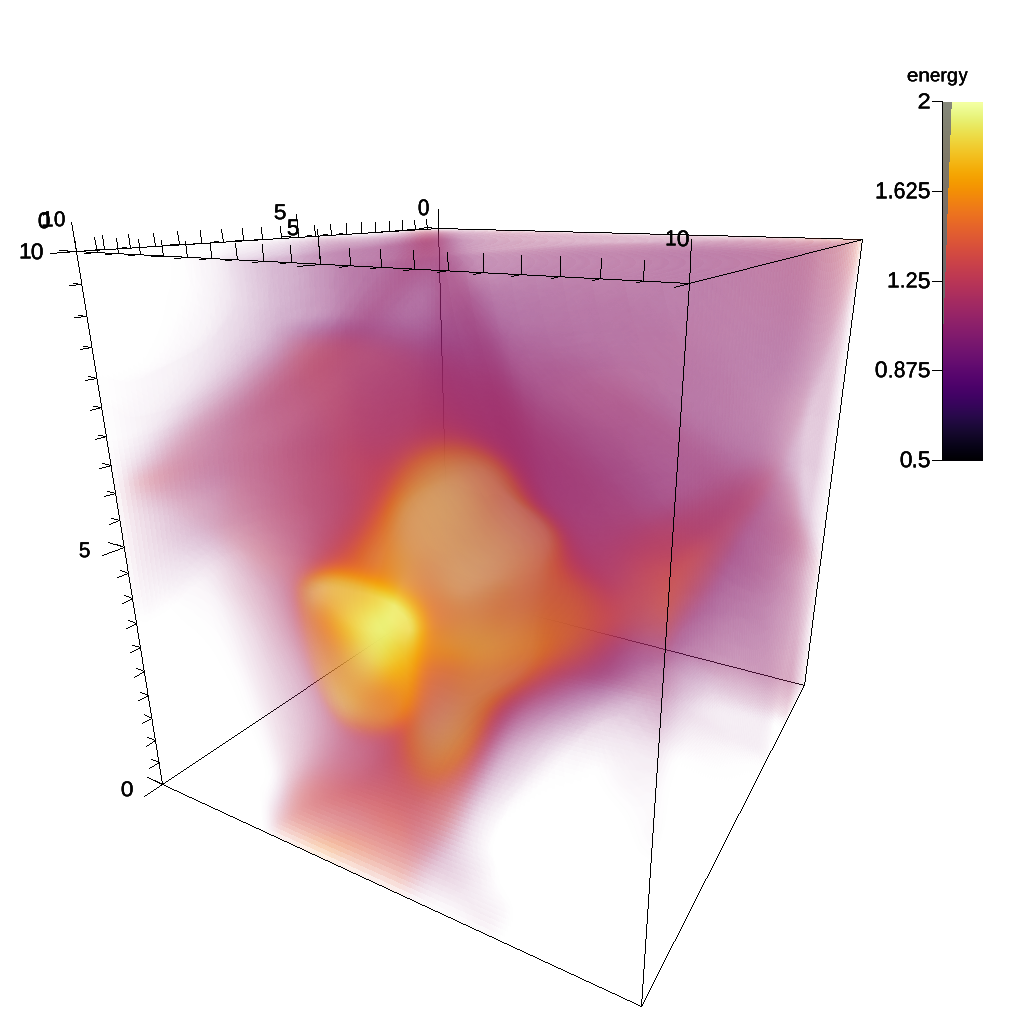
\includegraphics[width=0.4\textwidth]{images/volume250}
  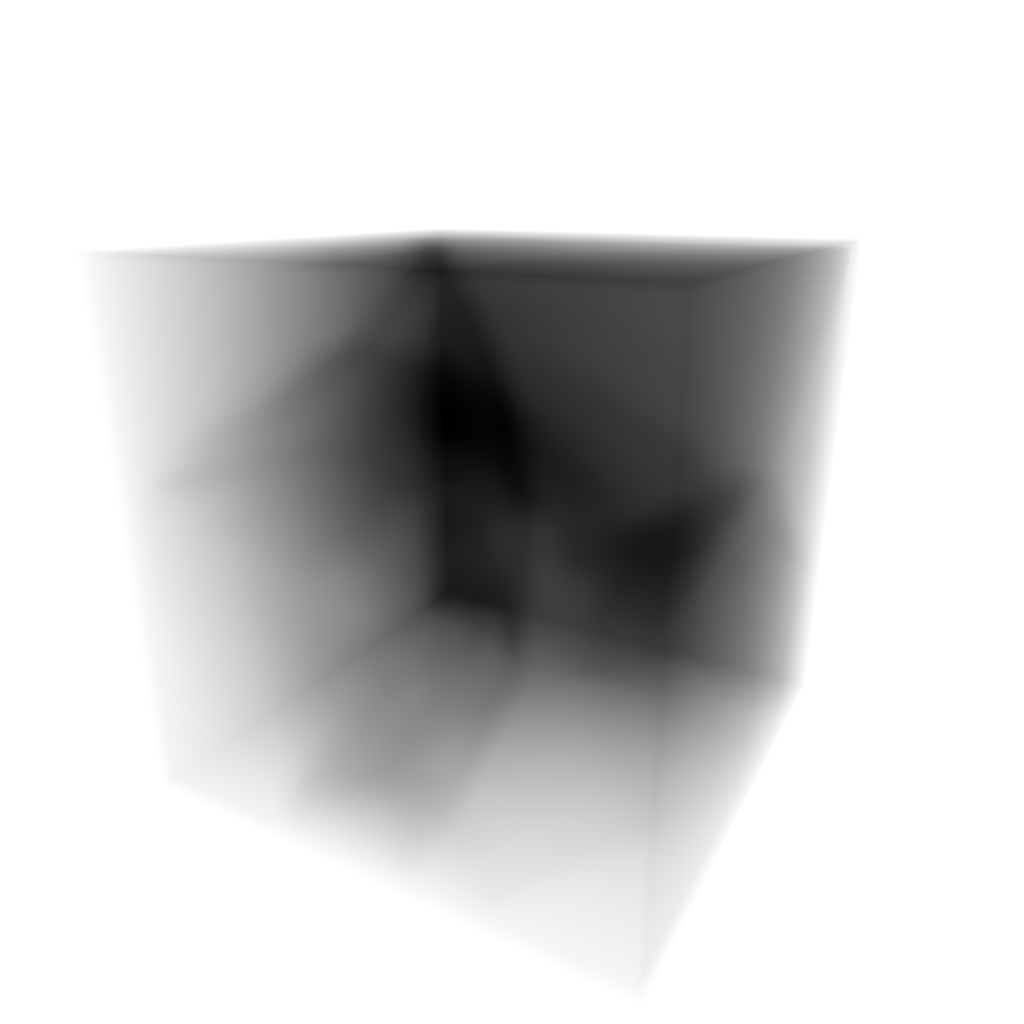
\includegraphics[width=0.4\textwidth]{images/radiograph250}
  \caption{\label{fig:ascent_plots} Example images of Ascent's four plot types:
pseudocolor (top left), mesh (top right, which also includes a pseudocolor plot),
volume rendering (bottom left), and radiograph (bottom right).
%
The data for these images comes from CloverLeaf3D, 
a hydrodynamics proxy-application included with Ascent.
  }
\end{figure}

In terms of camera placement,
Ascent creates a default camera based on bounding box of the data set 
that faces the data set.
%
Renders inherit the default camera parameters, simplifying creation of useful
cameras positions.
%
Ascent also provides simple controls to rotate the camera on the
sphere circumscribing the data set.
%
Of course, the user is free to set all
camera parameters explicitly as well.

Finally, scenes can create Cinema~\cite{AhrensCinema} databases, i.e.,
a large set of images that can be explored after the simulation.
\fix{Should be a reference to Cinema chapter here.}

%Currently supported plots include:
%\begin{itemize}
%\item Pseudocolor
%\item Mesh
%\item Volume
%\item Radiograph
%\end{itemize}

\subsection{Extracts}
The extracts action covers a broad range of activities.
%
The common theme between these activities is moving data outside Ascent.
%
The word extract is meant to convey ``extracting'' data from Ascent to somewhere else.
%
%
%Extracts are an escape hatch in Ascent that enables data to be sent
%outside of Ascent.
%
Extracts can be as simple a saving data to HDF5 files.
%
That said, extracts are also the mechanism to integrate other tools with Ascent --- a gateway
to a larger workflow.
%
This is important because
Ascent does not have the long tail of functionality that tools like ParaView or VisIt provide, which
were built over decades of development.
%
Through extracts, Ascent can pass data directly to ParaView Catalyst~\cite{Catalyst}.
%
Another example of using extracts to provide additional functionality is the
ADIOS~\cite{Lofstead2008} extract, which allows Ascent to link to in transit workflows.

Ascent supports connections to the Python ecosystem through its Python and
Jupyter extracts~\cite{CyrusISAV,Jupyter}.
%
Python extracts execute custom analysis code provided by the user, and the
Jupyter extracts allow for incoming Jupyter notebooks connections from a web
browser.

We feel that the Jupyter notebook interface is an important future direction
for Ascent, and for in situ as a whole.
%
One of in situ's greatest weaknesses is the reliance on a priori
knowledge, and one strategy to mitigate this weakness is incorporating a human-in-the-loop.
%
Through the Jupyter notebook interface, users can pause a running simulation
and interact with the data.
%
Additionally, Jupyter widgets enable fast prototyping of domain specific GUIs.

In all, currently supported extracts include:
\begin{itemize}
\item ADIOS
\item Babel Flow~\cite{babelflow}
\item Jupyter Notebooks
\item ParaView Catalyst
\item Python
\end{itemize}

\subsection{Queries}
\label{action_queries}
Queries enable users to ask quantitative questions.
%
The inputs to a query can take a varied form:
the simulation data directly,
data produced by a pipeline,
or even a combination of multiple pipelines and simulation data.
%
That said, typical queries are used to access the current state of the simulation
and to summarize data.
%
The results of queries are saved in Ascent's state.
%
These results can then be used to
interact with other actions --- a query's return value can be turned
into the parameter for another action (for example setting the camera position in a scene based
on the result of a bounding box query) or it can be used to affect triggers.
%

The mechanism behind queries enables powerful operations.
%
Queries are formed via a Python-like language that
enables expressions for math operations,
call functions, and evaluating conditionals.
%
Further, since the results of queries are stored into named identifiers, subsequent queries
can build on the results of other queries, allowing for complex combinations.
%
%Examples include min-max queries, statistics, cell locations,
%and probability distributions.
%
This also enables creating a ``time history,'' since
Ascent can call the same query every time step and accumulate the result.

%Queries are executed each time Ascent is called, and the resulting time
%history can be saved, accessed by the simulation, or accessed in other
%expressions.

%Queries can be as simple as calling a function that returns the current simulation cycle
%and storing it into a variable.
%
%More complex queries can calculate the amount of entropy of a field.
%

Examples of queries include:
\begin{itemize}
\item $cycle()$: calling a function that return the current simulation cycle and storing it into a variable.
\item $max(field('pressure'))$: the maximum value of the pressure field.
\item $entropy(histogram(field('gyre'), num\_bins=128))$: calculating a histogram of the gyre field with 128 bins, and then calculating the entropy of that histogram.
\end{itemize}
%Listing~\ref{simple_query} shows the declaration of a query that returns
%the current simulation cycle and stores it into a variable identifier \textit{cycle},
%and Listing~\ref{complex_query} shows a more complex example of a query that
%calculates the entropy of a simulation field.
%\begin{lstlisting}[language=Python,caption={Examples of querying the simulation cycle}, label={simple_query}]
%# add a simple query expression (q1)
%queries["q1/params/expression"] = "cycle()"
%queries["q1/params/name"] = "cycle"
%\end{lstlisting}
%

%
%
%\begin{lstlisting}[language=Python,caption={A more complex example of queries in Ascent}, label={complex_query}]
%# add a more complex query expression (q2)
%queries["q2/params/expression"] = "entropy(histogram(field('gyre'), num_bins=128))"
%queries["q2/params/name"] = "entropy_of_gyre"
%\end{lstlisting}

\subsection{Triggers}
\label{sec:ascent:triggers}

``Triggers'' are designed to balance the tensions between cost and capturing important phenomena.
%
In a typical scenario, in situ visualization is performed at regular intervals, e.g.,
every $X$ simulation cycles or every $M$ minutes of wall clock time.
%
This approach creates a tension between two important goals:
(1) achieving the visualizations and analyses at the right times within the simulation
and (2) minimizing costs.
%
On the one hand, performing visualization frequently maximizes the chances of having
visualizations at the right times (and likely also some uninteresting times), but
is costly,  e.g., adding a 50\% overhead on top of the simulation.
%
On the other hand, performing visualization infrequently minimizes costs, but also makes it
less likely that the visualizations will occur during important phenomena.
%

Triggers operate in two phases: inspection and action/inaction.
%
The purpose of the inspection phase is to determine if the action should be taken, if so, then
the trigger should ``fire.''
%
Further, if the inspection routine is cheap (i.e., executes quickly) and accurate (i.e.,
fires at the right times), then
triggers can be an effective strategy.
%
In this case, triggers can be called frequently (possibly every cycle) and still minimize cost
(since the visualization in the action/inaction phase is called only when necessary) and
get the right information (since the trigger is accurate).
%
Of course, triggers make the most sense when the desired visualization is quite expensive
to calculate;
if the desired visualization could be calculated as quickly as the inspection, then there would
not be a cost benefit.





%Traditional in situ actions execute every $X$ simulation cycles, this presents
%two related problems.
%
%First, if the analysis is expensive, then the total cost of the action may exceed
%what a user is willing to pay,
%
%Second, if the analysis called infrequently, then the feature or event that the analysis is
%trying to capture could easily be missed.
%
%Triggers address these issues by coupling inspection routines with analysis, and a
%potentially costly analysis only executes when user defined precondition is met.
%
%Ideally, inspection routines are cheap and can be called every cycle, while the analysis
%that are ``triggered'' can cost more.

A trigger is made up of two parts; for clarity, we term these two parts 
as trigger-condition and trigger-action.
(A trigger-action is only executed if the trigger-condition is true.)
%
In Ascent, any conditional expression can be a trigger-condition, although most trigger-conditions
incorporates the queries and expressions infrastructure from
\S\ref{action_queries}.
%
Trigger-actions utilize Ascent's other actions: pipelines, extracts, scenes, and
queries.  
%
For example, a trigger-action may be to calculate an isosurface (pipeline) and save
an image (scene).
%The part for the action incorporates 
%When the condition evaluates to true, the trigger fires, executing a user provided
%set of actions, which can be any Ascent action.
%
In practice, triggers are often used for debugging (e.g., saving data to
a file when invalid values are found) or 
for capturing information when a phenomena occurs
(e.g., saving an image when the maximum value of a field exceeds a threshold from the
previous value).
%
%When an event can be expressed in these terms, triggers are a powerful tool for
%maximizing constrained resources in situ.

Examples of trigger-conditions in Ascent include:
\begin{itemize}
\item $cycle() > 100 \ and \ cycle() < 200$
\item $max(field('pressure')) > 100.0$
\item $magnitude(max(field('braid')).position - vector(0,0,0)) > 0$
\end{itemize}

\subsection{Interactions Between Actions}

Although some of the interactions between Ascent actions have been mentioned previously,
this subsection formalizes and summarizes these interactions.
%
The key takeaway is that the Ascent project has smooth pathing between its actions.
%
This constrasts with other projects, where interoperability between different types of actions
can be difficult or impossible.

\begin{figure}
\centering
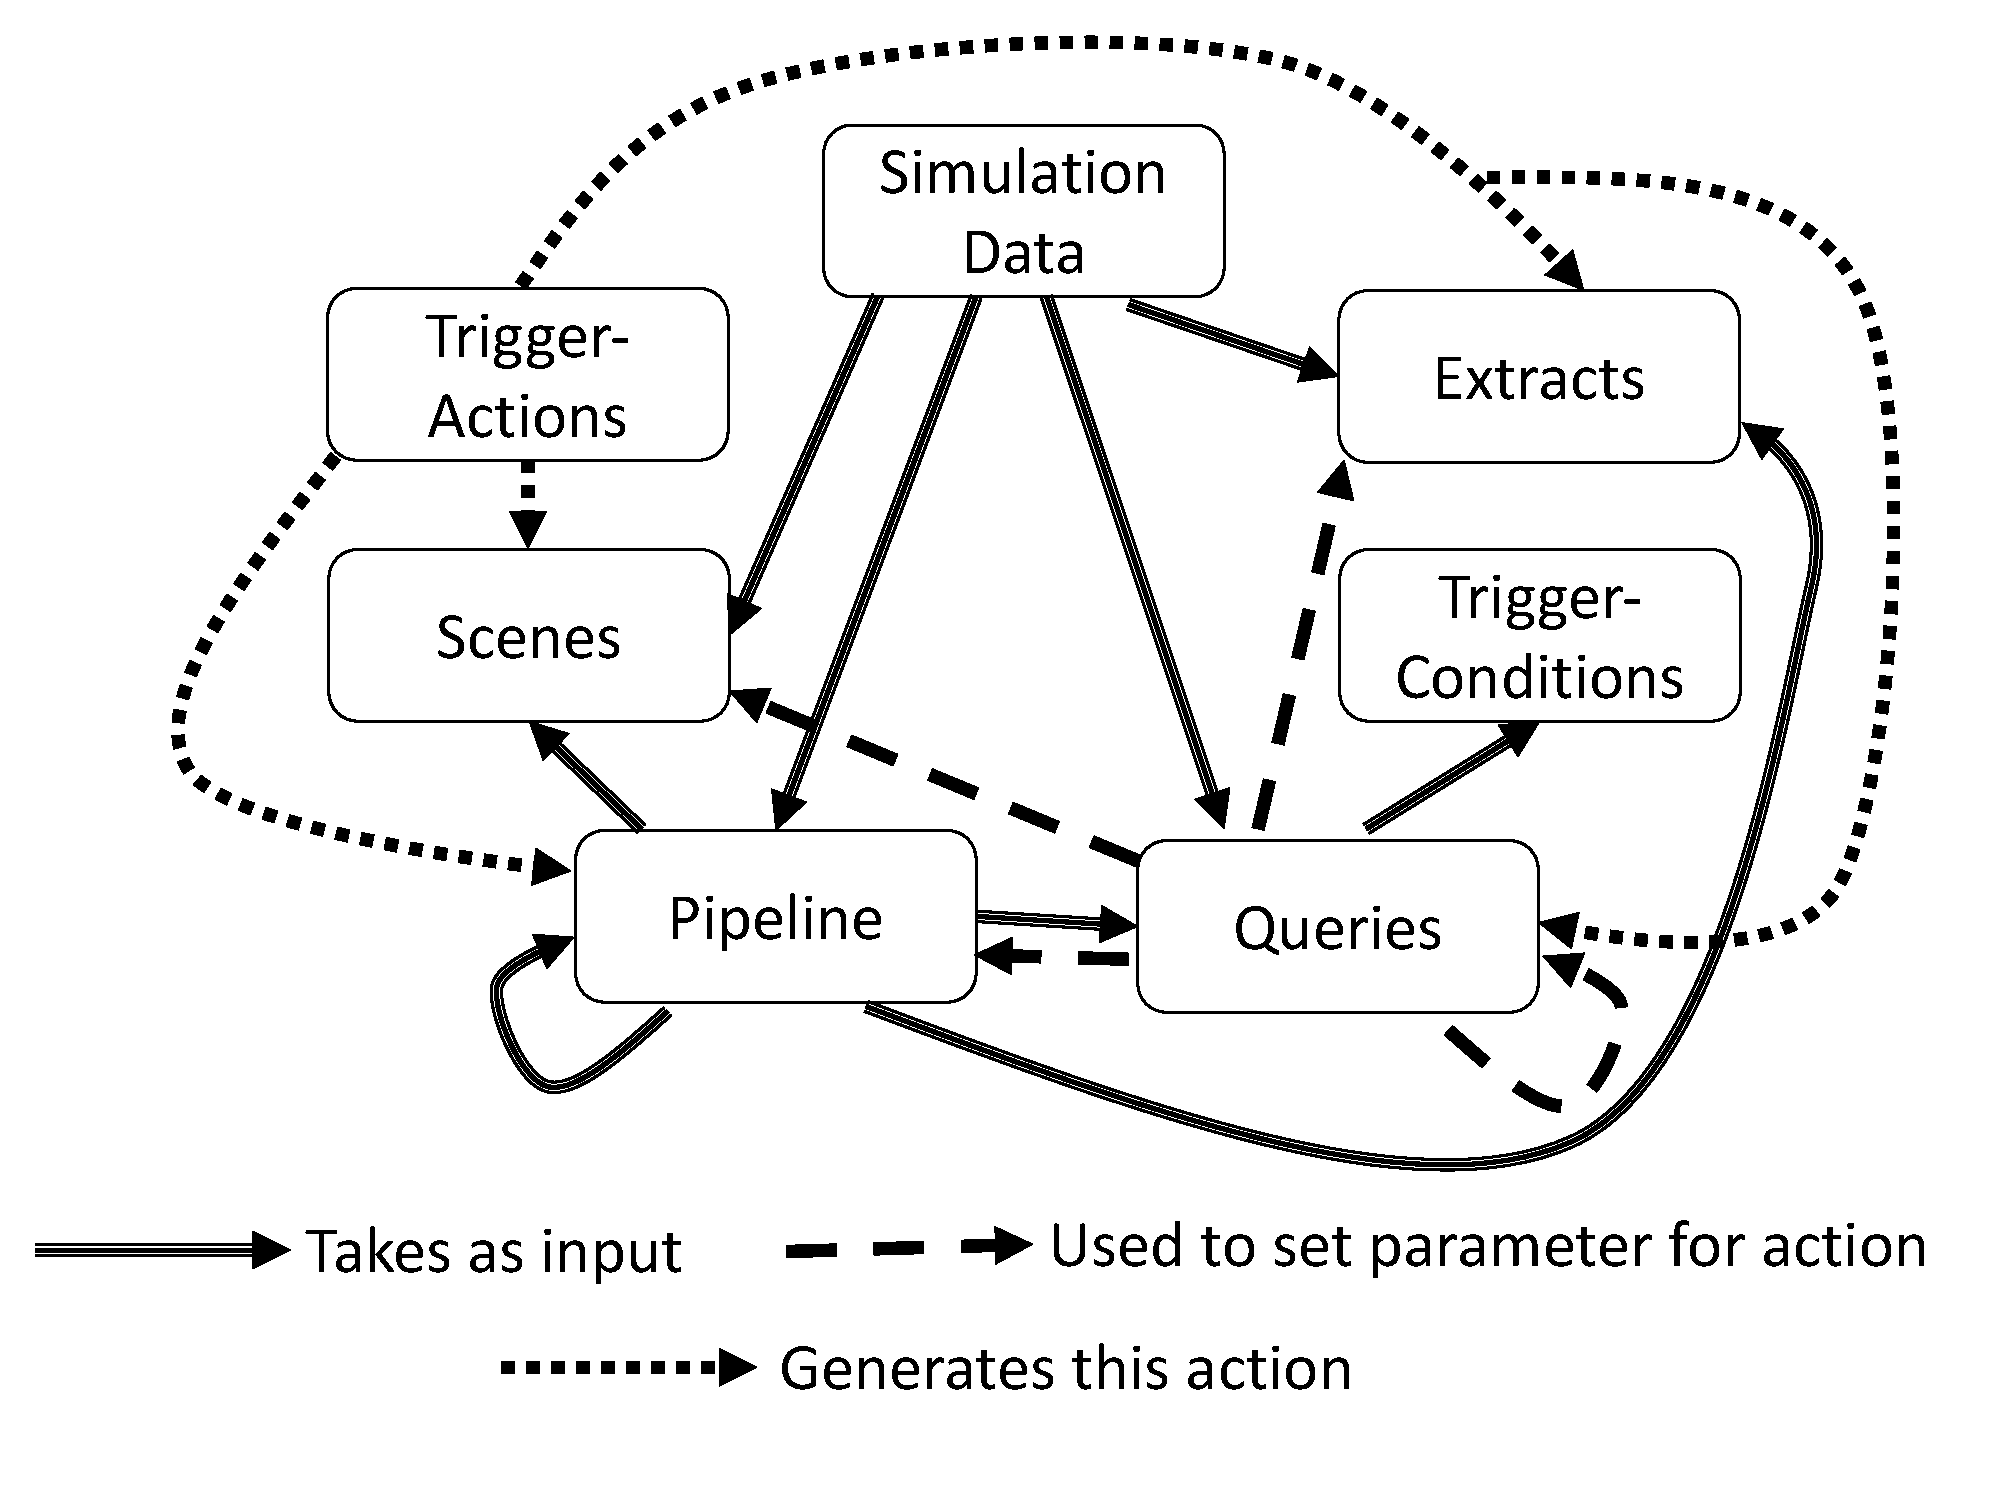
\includegraphics[width=0.75\textwidth]{images/ascent_interactions}
\caption{\label{fig:interactions} Interactions between Ascent actions.}
\end{figure}

Figure~\ref{fig:interactions} shows interactions between Ascent's actions.
%
It shows three types of interactions via arrow glyphs:
%
\begin{itemize}
\item Takes as input: the action at the tail of the arrow may serve as input for the action at the head of the arrow.
\item Used to set parameter for action: the action at the tail of the arrow may set parameter values for the action at the head of the arrow.
\item Generates this action: the action at the tail of the arrow may generate actions of the type at the head of the arrow.
\end{itemize}

Two of these interaction types are simply described.  
%
First, queries are the only action that can set parameters for other actions, and it does so for
pipelines, scenes, and extracts, as well as for other queries.
%
Second, trigger-actions are the only action that can spawn new actions, and the types it spawns are
pipelines, scenes, extracts, and queries.
%

The last interaction type is on inputs.
%
Simulation data is input to pipelines, scenes, extracts, and queries.
%
Pipelines are input to the same types of actions, meaning that pipelines can serve as input
to other pipelines.
%
Further, in these cases, there can be multiple inputs, e.g., one query can have multiple
pipelines as input.
%
The last input involves queries and trigger-conditions. 
%
In this case, the queries would have their own inputs (i.e., simulation data or pipelines), 
but the trigger-condition would be firing or not based on the result of the query ---
the simulation data or pipeline is one step removed.

Finally, Figure~\ref{fig:interactions} shows simulation data as only being at the tails of arrows,
and never the heads, i.e., nothing is ever sent to the simulation.
%
In reality, Ascent does have pathing to send data back to the simulation.
%
This is most useful for queries, but also applies to the other actions.
%
For example, it is possible to have a scene return an image (instead of writing it to disk)
and then pass that image back to the simulation (as bytes).




\section{System Architecture --- Matt}
\label{sec:design}
In the previous section, we described Ascent's high-level abstractions and
capabilities.
%
This section discusses Ascent's system architecture starting at its inner layer, Flow,
and moving outward.

\subsection{Flow: A data-type agnostic data-flow based architecture}
\label{sec:flow}
Ascent uses a graph-based data-flow architecture.
The data-flow architecture allows Ascent to track, re-use, and cleanup intermediate
results efficiently while implementing complex visualization pipelines.
The design also abstracts how we register and execute operations,
which simplifies adding new features.

At Ascent's core is a simple data-flow library known as Flow, that
composes and executes filters, which are the basic unit of execution in Ascent.
%
Flow is an evolution of a Python data-flow network
~\cite{flow_reference}, but unlike its ancestor, Flow is a C++
library.
%
Flow supports composing and executing directed acyclic graphs
(DAGs) composed of filters~\cite{LarsenAscent}.

There are four components to Flow:
\begin{itemize}
  \item \textbf{Filter}: basic unit of execution.
  \item \textbf{Graph}: contains the filter graph and manages the adding of
filters.
  \item \textbf{Registry}: manages the lifetime of filter results.
  \item \textbf{Workspace}: contains both the registry and filter graph,
coordinates graph execution.
\end{itemize}

\paragraph{Flow Filters}
Flow filters are the basic unit of execution inside of Ascent, and
almost all functionality inside of Ascent is implemented as a Flow filter.
%
Adding new capabilities to Ascent means wrapping that functionality inside
a flow filter.
%
Filters declare an interface, i.e., how many inputs a filter has and
if there is an output, and filters are passed a set of parameters inside
of a Conduit node (see \S\ref{Conduit}).
%
Filter inputs are tracked as arbitrary pointers and runtime features allow
filters to identify and obtain concrete types for processing.
%
In terms of Ascent actions, pipeline filters become part of a chain of
data transformations and would minimally have an input
data set and an output data set, while scenes and extracts
become sinks that have an input data set and no output.
%

\paragraph{Graph}
The graph is a series of Flow filters connected together into
a DAG.
%
The graph is responsible for storing filters and connections
between filters.
%
The primary graph interface supports adding filters and connecting
filter ports (e.g., inputs and outputs) together.

\paragraph{Registry}
The registry is a key-value data store used to manage the intermediate
results of filters inside the data-flow network.
%
Keys within the registry are reference counted, and data contained
inside the registry is deleted when the reference counts reach zero.
%
While the data associated with a key can be a pointer to any type,
the majority of the data stored in the registry are Conduit Nodes
or VTK-m data sets.


\paragraph{Workspace}
The workspace is a container for both the graph and the registry,
and the workspace is responsible for executing the DAG.
%
Additionally, the workspace manages the lists of known filters.
%
A filter must be registered with the workspace in order to be added to the
graph, and once registered, a filter can be added to the graph by name.
%
Flow uses a topological sort to ensure proper filter execution order,
to track all intermediate results, and to provide basic memory management capabilities.
During execution, the workspace provides the registry with reference counts that reflect graph connections, allowing intermediate results to be efficiently managed.

%
Multiple workspaces can co-exist, and in fact, Ascent uses a separate Flow workspace
to evaluate expressions within the Ascent runtime.
%

\subsection{Runtime}
The Ascent runtime builds on top of Flow, and the main responsibility of the
runtime is to translate user actions into data-flow networks.
%
For example, when a user describes a series of data transformations inside of a pipeline,
the runtime adds the corresponding filter for each transformation to
the internal Flow graph.
%
Some actions, like the contour filter, have exactly one filter that the runtime
adds when translating actions, while other actions add more than one filter to the graph.
%
Fig.~\ref{img:flow_graph} shows a simplified view of a data-flow network constructed by the
runtime to create contours of a simulation field and rendering an image of the result.
%

\begin{figure}
\centering
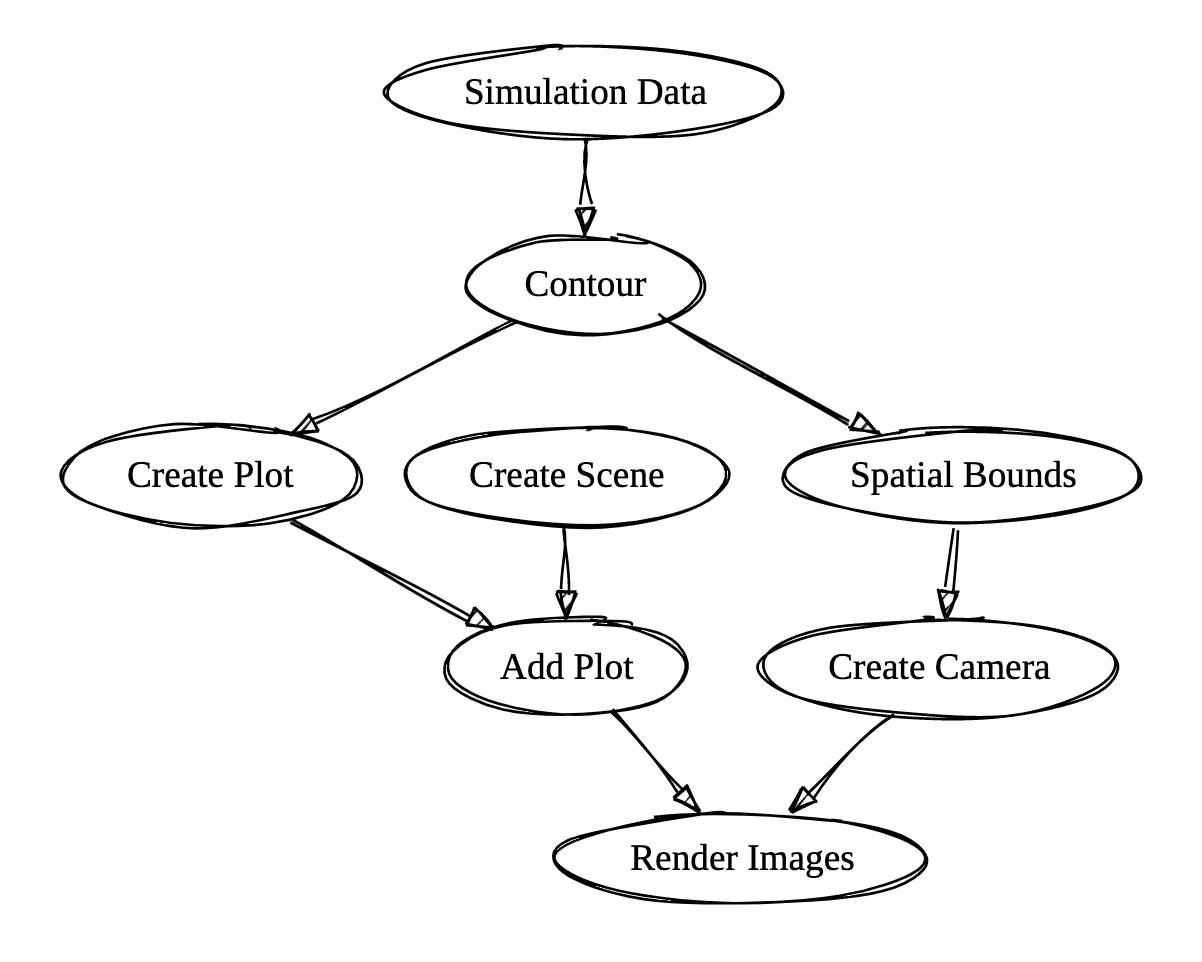
\includegraphics[width=0.6\textwidth]{images/flow_graph}
\caption{\label{img:flow_graph} An example data flow network using Flow assembled by the Ascent runtime.}
\end{figure}

Internally, the runtime maintains a list of registered filters to map
user-facing API names to the corresponding Flow filters which are hidden
from the user.
%
In addition to mapping API calls to Flow filters, the filter map also specifies
in what actions a filter can be used.
%
Runtime Filters can be registered as either a ``transform'' or an ``extract.''
%
Transforms are only callable inside of pipelines and extracts can only be called at the end of a pipeline.
%
Built-in functionality is registered internally with the Ascent runtime when Ascent is initialized.


The runtime also exposes the filter registration of the underlying data flow network which
allows the runtime to inherit Flow's flexibility.
%
Simulations, or other analysis libraries, are free to register custom capability at
runtime, and this allows outside functionality to build off the capability
provided by Ascent.
%
Just like internal filters, custom filters can either be registered as transforms or extracts,
and can directly connect with simulation data or consume the results of a pipeline.
%

The other responsibility of the runtime is to interface with the simulation through Ascent's
main API calls.
%
The runtime consumes configuration options like MPI communicators, exception
handling, and what
backends (e.g., OpenMP or CUDA) to execute code on.
%
Additionally, the simulation's mesh data and the actions are all passed to the runtime.

\subsubsection{Parallelism in Ascent}
Ascent is a hybrid-parallel library, meaning that it uses both
distributed-memory (e.g., MPI) and shared-memory parallelism
(e.g., CUDA and OpenMP), and Ascent is primarily
tightly-coupled with simulations.
%
In the tightly-coupled paradigm, simulations control how parallelism is used, so
it is imperative that Ascent's functionality be capable of running
on the same architectures using the same types of parallelism as the
simulations.
%
Ascent supports many different parallel configurations including
one MPI rank per core (i.e., no shared-memory parallelism), one rank
per GPU, and one rank per node.
%
While Ascent does internally leverage shared-memory parallelism
for expressions, the majority of the shared-memory parallelism comes
from Ascent's components such as VTK-m and Devil Ray.

\paragraph{Distributed-Memory Parallelism}
Within Ascent, all MPI ranks receive the same set of actions.
%
Since the actions are the same, all MPI ranks create and execute the same graph,
meaning that all flow filters execute on all ranks.
%
Ascent guarantees that each filter is given full control of MPI communication,
and filters are free to use MPI anyway they see fit, including
creating asynchronous tasks.
%
Some filters, such as threshold, do not need to use any
MPI communication, i.e., each block of data is processed independently,
but other filters, such as particle advection, use MPI to pass particles
from one rank to another.
%
For mesh data, as discussed in \S\ref{ascent_control},
each MPI rank receives data published by the simulation, and
Ascent does not redistribute the data.
%
That said, filters can change the data distribution (e.g., resampling
an unstructured grid onto a uniform grid), although this can be a costly
operation.
%

\paragraph{Shared-Memory Parallelism}
Ascent's main components use portable performance abstraction layers to
take advantage of the different types of shared-memory parallelism on
modern supercomputers.
%
For example, VTK-m is itself a portable performance layer designed specifically
for visualization and currently supports OpenMP, CUDA, and TBB.
%
Devil Ray, while not itself a portable performance layer, uses RAJA to execute
on different architectures, supporting OpenMP, CUDA, HIP, and TBB.

\subsubsection{Data Set Representations}
Ascent uses an internal data abstraction, called the data object, as the input
and outputs of filters.
%
The data object is responsible for transforming data from one in-memory format
to another without unnecessary copies.
%
By using this abstraction, filters can ask for whatever data set
representation they need, however, the conversions between data
representations are not always one-to-one and may not always
result in a shallow copy.
%

To support multiple data set representations, there must be a common
set of supported features, but not all data models Ascent uses
support the same set of features.
%
Since Ascent uses Blueprint(see \S\ref{Blueprint}) as its data interface to simulations,
all other data models must sometimes be adapted to support additional
features.
%
For example, Blueprint supports multiple topologies in the same data set
but VTK-m only supports a single topology.
%
To handle this correctly within Ascent, we wrap the data sets in a container
that treats each topology as individual VTK-m data sets.
%


\section{Ascent APIs --- Hank}
\label{sec:API}

\section{Success Stories --- Matt}
\label{sec:success}
\subsection{In situ visualization of an Inertial Confinement Fusion (ICF) simulation}

Ascent was used to visualize the results of an unprecedented 3D simulation
of two-fluid mixing in a spherical geometry to better understand hydrodynamic
instability and the transition to turbulence process that is important to
the field of inertial confinement fusion and High Energy Density (HED)
Physics. High resolution simulations of instability growth are not practical
for routine use, so high resolution simulations like this help guide the
development of sub-grid models that capture instability effects with much
less computational cost, which are used for ICF calculations.

\begin{figure}
\centering
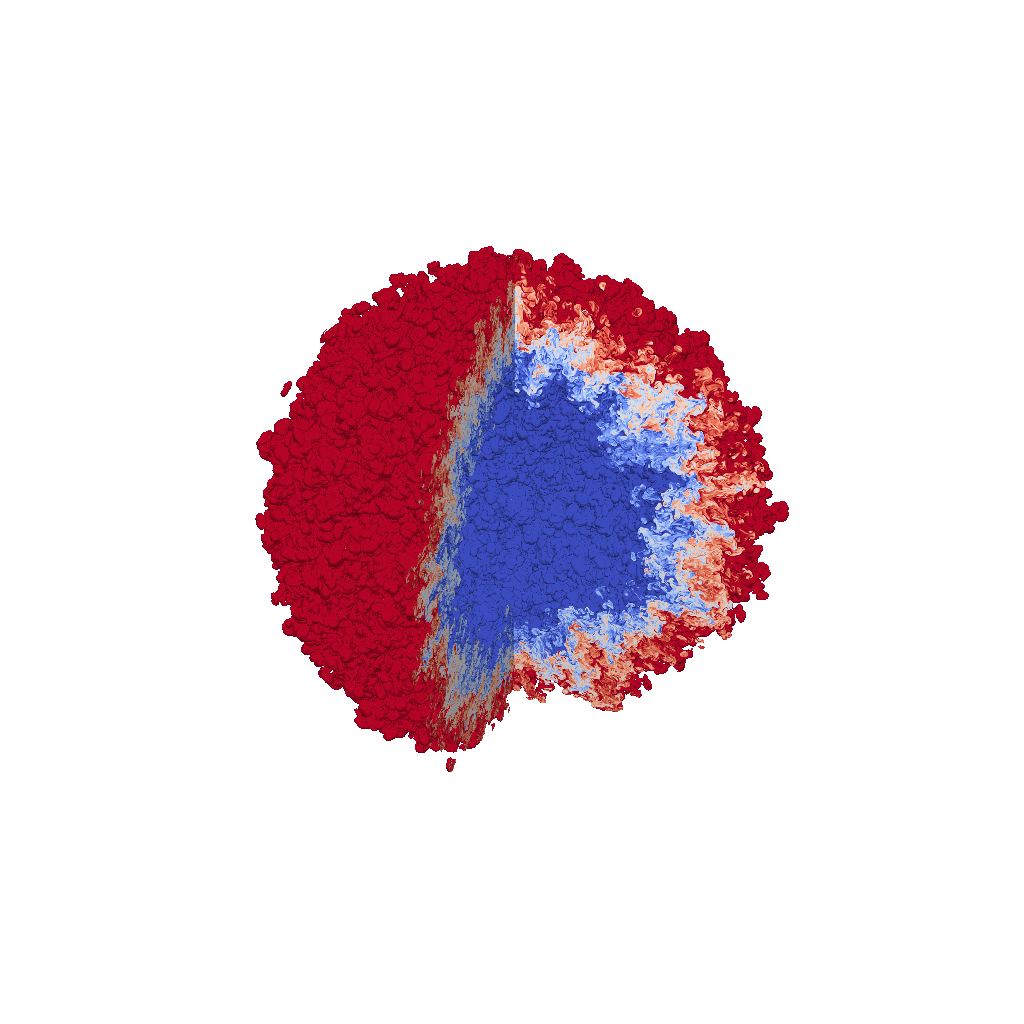
\includegraphics[trim={ 0 8cm 0 7cm},width=0.9\textwidth]{images/mixing_ball}
\caption{\label{img:icf}
This image is of an idealized Inertial Confinement
Fusion (ICF) simulation of a Rayleigh–Taylor instability
with two fluids mixing in a spherical geometry.
An isovolume filter was used to show only the mixing region of the heavy and
light fluids, and the a clip filter was added to show the internal of the sphere.
}
\end{figure}

The simulation was run on the Lawrence Livermore National Laboratories(LLNL)
Sierra system, a 125 Petaflop peak system from IBM that has 4,320 nodes,
each with 2 IBM POWER9 processors, 4 NVIDIA Tesla V100 GPUs, 320 GiB of
fast memory (256 GiB DDR4 memory and 64 GiB HBM4), and 1.6TB of NVMe
memory. The specific simulation was a 97.8 billion element simulation
run across 16,384 GPUs on 4,096 compute nodes. The simulation application
used CUDA via RAJA to run on the GPUs. The time-varying evolution of the
mixing was visualized in situ with Ascent, also leveraging 16,384 GPUs.
The last time step was also exported by Ascent to the parallel file
system for detailed post-hoc visualization using VisIt. The simulation
data was accessed by Ascent directly from the GPU memory, eliminating any
extra data copies.
Figure~\ref{img:icf} shows one of the many images generated in situ during
this run.

\subsection{MARBL Simulation Integration}
Ascent has been integrated and released with LLNL's MARBL simulation code,
a new next-generation multiphysics code currently under development.
%
One of MARBL's components is a high-order finite element solver build on
MFEM, and Ascent supports the MFEM data model.
%
In order to leverages Ascent's visualization capabilities, Ascent refines
the high-order elements to low-order(i.e., linear elements).
%
Ascent can be activated through the simulation's input deck, and in addition
to adding in situ visualization capabilities, Ascent can be used to save out
the mesh and only the fields that the user specifies.
%
Previously, MARBL only saved out full checkpoints, and only saving a subset of the
data allows users to save data for post-hoc analysis at much higher temporal resolution.

As a new code, simulation validation plays an important role, and one method
for simulation validation is comparing the results of experimental data to the
simulated experiments.
%
One such experiment is a radiation driven Kelvin-Helmholtz shear
layer experiment~\cite{hurricane2009high}.
%
The experiment captured radiographs of the instability as it was driven through
the material, and comparing experimental radiographs with radiographs created from
the simulation are a useful simulation validation tool.
%
MARBL ran a simulation of this problem using 2304 MPI ranks for 120 hours.
%
Figure~\ref{img:radkh} shows a volume rendering and simulated radiograph
generated as a result of this simulation.
%
\begin{figure}
\centering
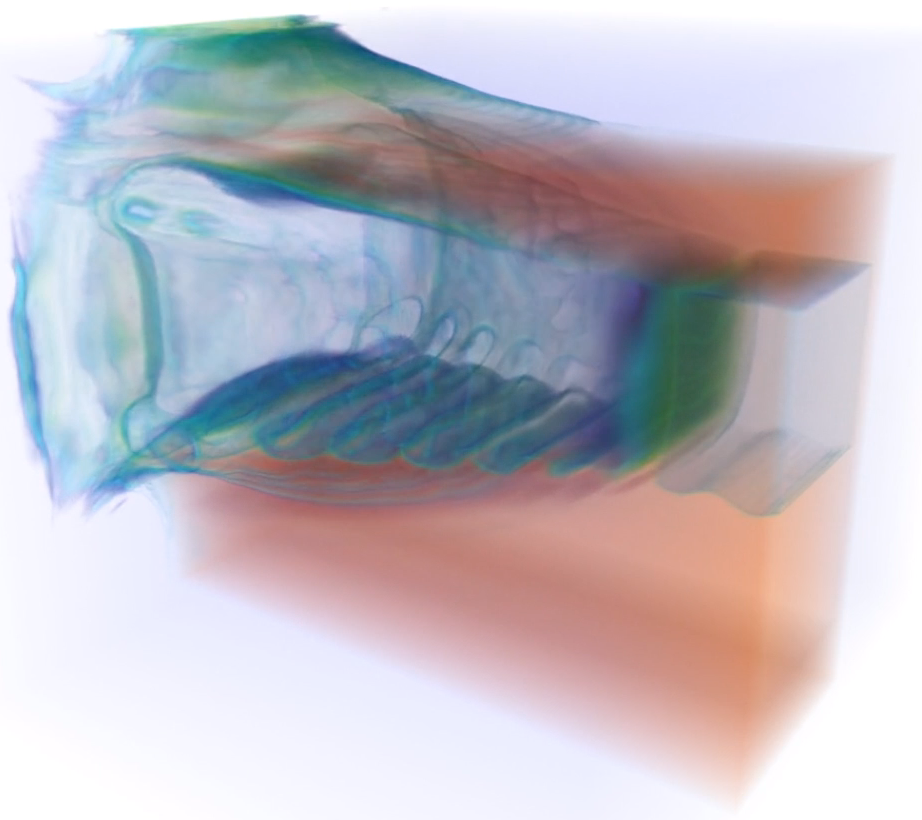
\includegraphics[width=0.4\textwidth]{images/radkh}
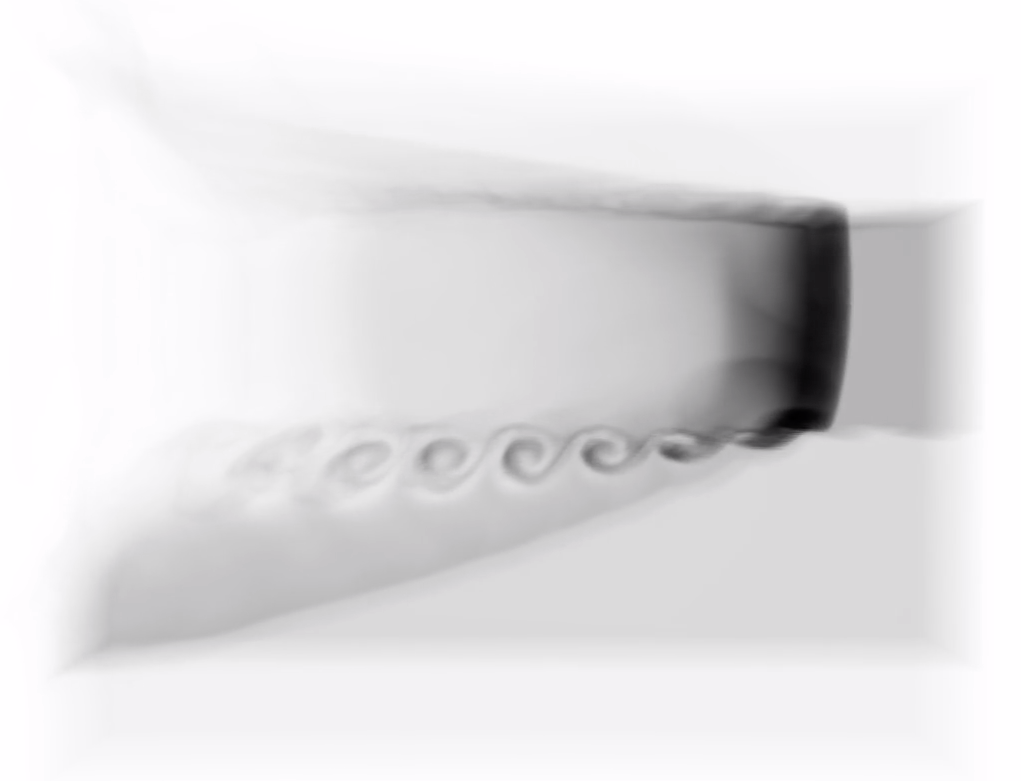
\includegraphics[width=0.4\textwidth]{images/radkh_xray}
  \caption{\label{img:radkh}A volume rendering(left) and simulated radiograph(right) created by
Ascent during a Kelvin-Helmholtz simulation.}
\end{figure}

%\subsection{Integrations}
%
%\begin{itemize}
%\item MARBL
%\item ARES
%\item AMRex: Warpx, Pele, NYX
%\item SW4
%\end{itemize}





\subsection{Devil Ray Rendering}
\label{sec:DevilRay}

\fix{EVERYTHING BELOW THIS POINT IS CURRENTLY ORPHANED.  AUTHORS
SHOULD PULL INFORMATION FROM THE BELOW AS THEY POPULATE THE SECTIONS
ABOVE.}


\if 0
Statement about capabilities.  Emphasis on being an integrator.
This is where Jupyter, triggers, etc. get mentioned.  Also emphasize
exascale.
Ascent has a rich feature set and integrates with other ecosystems.

\begin{itemize}
  \item Supports common visualization operations such as slicing and dicing your data.
  \item Supports ray traced surface and volume rendering as well as simulated radiography.
  \item Supports Queries for getting quantitative answers to questions
  \item Supports Triggers for adaptive visualization and analysis
  \item Outputs images sequences and Cinema image databases
  \item Outputs extracts for exporting data to HDF5, ADIOS, Python and Jupyter
  \item Support interactive visualization and analysis with Jupyter and Catalyst
  \item Supports C/C++, Python and Fortran language bindings
\end{itemize}

Statement about Devil Ray, but a forward reference a section in success stories --- success as an integrator.
\fi


\section{The Ascent In Situ Infrastructure}
\label{ascent_overview}
%Use the template \emph{chapter.tex} together with the document class SVMono (monograph-type books) or SVMult (edited books) to style the various elements of your chapter content conformable to the Springer Nature layout.

%List how ascent makes things easy.

\section{Design Considerations}
\label{ascent_design_considerations}

\subsection{Reduce required dependencies and adhere to a lightweight memory footprint}
Software complexity. Ascent is less complex.

\subsection{Target exascale architectures: maximize constrained resources}
Ascent's primary in situ use case is tightly-coupled, i.e.,
Ascent shares the same computational resources (proximity) and
memory space as the simulaiton (access).
%
All core functionality in Ascent, transforming data
and making pictures, executes on the same hardware as the
simulation through portably performance abstractions such as
VTK-m and RAJA.
%
This enables Ascent to minimize data movement by directly accessing
the simulation data memory without making copies of the data.
%

Memory and time are both constrained resources in situ.

%
Simulations often consume almost all availble system memory,
leaving only a small fraction to in situ infrastructures.
%
It is imperative that Ascent uses memory as efficiently as possible
as not to exceed system memory.
%
To that end, Ascent can directly access simulation memory, whether it be
on the CPU or GPU.
%
While important, direct simulation memory access is only half
the battle of memory efficiency.
%
Visualization pipelines transforms data(e.g., isocontours) from
one form to another, and efficiently managing the memory consumed
by intermediate results is equally important.
%
\fix{possible example: contour of turbulence simulation on
structured grid can create a dataset larger than the original.}
%
In Ascent, we free memory used by intermediate results as soon
as they are not needed by downstream transforms.
%


%
Supercomper architectures have significanlty changed since
%
Current community visualization tools, such as ParaView and VisIt, were originally
designed to execute using one MPI rank per CPU core.
%

All core functionality(i.e., transforming data and making pictures) in
Ascent targets exascale architectures.

VTK-m, devil ray

\subsection{Provide simple and flexible data and control interfaces}

\subsection{Create tools to address in situ resource constraints , e.g., a flexible trigger system that allows users to express what is important}

\subsection{Simplify connection to other ecosystems, e.g., python, custom analysis, and Juptyer Notebooks}



\section{Data Interface}
\label{ascent_data}
\subsection{Conduit: A foundation for in-memory data exchange}
\label{sec:conduit}
Conduit is a library that provides an intuitive model for describing
hierarchical scientific data in C++, C, Fortran, and Python.
%
The API is a JSON-inspired data model for describing hierarchical
in-core scientific data.
%
While primarily used for data coupling between packages in-core,
Conduit also provides easy access to serialization and I/O functions.
%
In this section, we will discuss some of the basics of Conduit
and describe the concepts needed to couple simulation mesh
data structures using Conduit's Mesh Blueprint.

\fix{At the end, we should mention how simulations codes are using conduit as
a central data store, and for checkpoints. It also might be nice to
illustrate some other interesting use cases like neurons, or diffing nodes
to update rendering states in wolf vision. The limits of using using Conduit
are only bounded by the imagination of the person who wields Conduit.}

\subsubsection{Conduit Basics}
The primary Conduit data structure is a Node.
%
Nodes stores data through a key-value interface.
%
Figure~\ref{ex:1} shows how to store a string ``value'' into a Node
with the key ``key''.

\begin{figure}
\begin{tabular}{cc}
  \begin{minipage}{.5\textwidth}
  \centering
    \begin{lstlisting}[language=C++]
Node n;
n["key"] = "value";
n.print();
    \end{lstlisting}
  \end{minipage}
  &
  \begin{minipage}{.5\textwidth}
  \centering
  \begin{lstlisting}[language=C++]
{
  "key": "value"
}
  \end{lstlisting}
  \end{minipage}
\end{tabular}
\caption{\label{ex:1}On the left, an example of storing a string inside a Conduit Node. On the right, the JSON equivalent.}
\end{figure}

Data in Nodes can be created and accessed through hierarchical keys,
and the key string looks much like a UNIX directory structure.
%
Key paths are completely up to the user.
%
Figure~\ref{ex:2} illustrates creating a Node hierarchy
and storing a floating point value in a leaf Node.
%
In this example, several Nodes are actually created with parent child
relationships defined by the key.
%
Node $n$ has a child Node $dir1$, which in turn has a child $dir2$,
and the tree ends at the leaf Node $val1$, which stores the data.
%
Nodes can contain many basic data types such as strings,
floating point values, and integers.

\begin{figure}
\begin{tabular}{cc}
  \begin{minipage}{.5\textwidth}
  \centering
    \begin{lstlisting}[language=C++]
Node n;
n["dir1/dir2/val1"] = 100.5;
n.print();
    \end{lstlisting}
  \end{minipage}
  &
  \begin{minipage}{.5\textwidth}
  \centering
  \begin{lstlisting}[language=C++]
{
  "dir1" :
  {
    "dir2" :
    {
      "val1": 100.5
    }
  }
}
  \end{lstlisting}
  \end{minipage}
\end{tabular}
\caption{\label{ex:2}On the left, an example of using a hierarchical key to store a number. On the right, the JSON equivalent.}
\end{figure}

Nodes can also contain arrays, and the $set$ method
copies the values from an array into a Node.
%
Figure~\ref{ex:3} shows how to set a Node to the contents of an array.
%
Alternatively, the $set_external$ copies only the pointer(i.e., a shallow copy),
and any change to the underlying array would be reflected in both the original
array and the data contained inside the Node.
%
Using $set_external$ is desirable for large data, such as simulation mesh data,
and in environments where memory is constrained.

\begin{figure}
\begin{tabular}{cc}
  \begin{minipage}{.5\textwidth}
  \centering
    \begin{lstlisting}[language=C++]
const int size = 4;
int A[size] = {0, 1, 2, 3};
Node n;
n["my_array"].set(A, size);
n.print();
    \end{lstlisting}
  \end{minipage}
  &
  \begin{minipage}{.5\textwidth}
  \centering
  \begin{lstlisting}[language=C++]
{
  "my_array" : [0, 1, 2, 3]
}
  \end{lstlisting}
  \end{minipage}
\end{tabular}

\caption{\label{ex:3}On the left, an example of setting the value of a Node to an Array. On the right, the JSON equivalent.}
\end{figure}

\subsection{Mesh Blueprint: An in-memory mesh description interface co-designed with simulation applications
System Architecture}

The flexibility of the Conduit Node allows it to be used to represent a
wide range of scientific data.
%
Unconstrained, this flexibly can lead to
many application specific choices for common types of data that could
potentially be shared between applications.

The goal of Blueprint is to help facilitate a set of shared higher-level
conventions for using Conduit Nodes to hold common simulation data structures.
%
The Blueprint library in Conduit provides methods to verify if a Conduit
Node instance conforms to known conventions, which we call protocols.
%
It also provides property and transform methods that can be used on conforming Nodes.

Many taxonomies and concrete mesh data models have been developed to allow
computational meshes to be used in software.
%
Blueprint’s conventions for representing mesh data were formed by negotiating
with simulation application teams at LLNL and from a survey of existing
projects that provide scientific mesh-related APIs including: ADIOS, Damaris,
EAVL, MFEM, Silo, VTK, VTKm, and Xdmf.
%
Blueprint’s mesh conventions are not a replacement for existing mesh data
models or APIs.
%
Our explicit goal is to outline a comprehensive, but small set of options
for describing meshes in-core that simplifies the process of adapting data
to several existing mesh-aware APIs.

Blueprint covers a wide range of mesh desriptions, and
Blueprint uses four concepts to describe meshes:

\begin{itemize}
  \item Coordinate Sets
  \item Topologies
  \item Fields
  \item Domain Decomposition Information
\end{itemize}

Coordinate sets described coordinate systems in 1D, 2D, and 3D, and
can be specified in cartesian, spherical, or cyclidrical frames of reference.
%
In additon to explicit coordinate sets, compact implicit representations,
such as uniform and rectilinear, are also supported.
%
Topologies describe the topological structure of the mesh elements.
%
As with coordinate sets, both implicit(e.g., uniform) and explicit
(e.g., completely unstructured)topologies are supported.
%
Fields describe the data associtate with the mesh, and Blueprint supports
fields associated with verticies or elements.
%
Fields can be scalars or have multiple components.
%
Additionally, Blueprint supports the description of high-order
topologies and fields, which are becoming increasingly common.

A Blueprint data set minimally needs a topology and a coordinate system,
but Blueprint supports having any number of topologies and coordinate
systems.
%
Figure~\ref{ex:blueprint} shows a Blueprint description of a uniform mesh.

\begin{figure}
\begin{lstlisting}[language=C++]
Node mesh;
// 10x10x10 uniform cooridinate system
mesh["coordsets/my_coords/type"]="uniform";
mesh["coordsets/my_coords/dims/i"] = 10;
mesh["coordsets/my_coords/dims/j"] = 10;
mesh["coordsets/my_coords/dims/k"] = 10;

// optional origin
mesh["coordsets/my_coords/origin/x"]= -10;
mesh["coordsets/my_coords/origin/y"]= -10;
mesh["coordsets/my_coords/origin/z"]= -10;

mesh["coordsets/my_coords/spacing/dx"]= 1.0;
mesh["coordsets/my_coords/spacing/dy"]= 1.0;
mesh["coordsets/my_coords/spacing/dz"]= 1.0;

mesh["topologies/my_topo/type"] = "uniform";
mesh["topologies/my_topo/coordset"] = "my_coords";
\end{lstlisting}
\caption{\label{ex:blueprint}An example of a specifying a $10^3$ uniform grid in Blueprint.}
\end{figure}


\section{Control Interface}
\label{ascent_control}
Ascent's control interface consists of two main components:
the API and actions.
%
The API is primaraly for getting data in and out of Ascent,
and the actions describe what to do with the simulation data
and what the simulation expects in return.

\subsection{Ascent API}
Ascent's front facing API consistst of five calls:
open, pushlish, execute, info, and close.
%
Ascent supports multiple language binding including C, C++,
Fortran, and Python.

%\begin{itemize}
%  \item open: initializes Ascent
%  \item publish: set the simulaiton data set
%  \item execute: performs a set of actions on the data set
%  \item info: returns information back to the simulation
%  \item close: cleans up Ascent
%\end{itemize}

\begin{lstlisting}[language=C++,caption={This cool caption}]
conduit::Node options, actions, data_set, info;
// fill options, actions, and data_set
ascent::Ascent ascent;
ascent.open(options);
ascent.pubish(data_set);
ascent.exectute(actions);
ascent.info(info);
ascent.close();
\end{lstlisting}

``open'' initializes ascent with a number of options including the
MPI communicator, exception handling, and the actions file name.
%
``publish'' takes in a Conduit Node containing the computational
mesh described using Blueprint.
%
``execute'' also takes in a conduit node containing the actions to
perform.
%
Typically, the parameters to ``exectute'' are overrided with a user provided
file, which allows actions to be changed without re-compiling the simulation.
%
``info'' is the mechanism for getting data out from Ascent into the simulation.
%
The Node passed to ``info'' is populated with data that includes the results
of queries, allowing the the simulation to take actions based on the results.
%
``close'' directs Ascent to finalize execution.


\subsection{Ascent Actions}
In Ascent, actions are a declarative interface that enables users to
control Ascent's exectution using five high-level concepts:
Pipelines, Scenes, Extracts, Queries, and Triggers.
%
Pipelines describe a series of data tranfomations, e.g.,
clipping and contouring.
%
Scenes describe the images to be rendered, consisting of one or more
plots (e.g., pseudocolor or volume rendering).
%
Extracts are a way to to get data out of Ascent and into other softeware
ecosystems, such as python.
%
Queries are a way to ask questions about the simulation data over time, and
the results are available to the simulation.
%
Triggers describe conditional actions based on simulation state and are a way
to create adaptive workflows inside of Ascent.

Under the hood, tools like ParaView and VisIt construct data-flow networks
to execute commands issued by the user through the GUI.
%
Abstractly, Ascents actions are a level below a GUI but at a higher level
than assembling a data flow network from scratch.
%
Constructing actions provides the user greater control and understanding
of exactly what is executing in situ, while still affording a higher level of
useability than programming directly in somnething like VTK.
%
Additionally, many filters in Ascent provide \textit{relative}
parameters so the user doesn't need to explicitly know filter parameter values
before the simulation executes.
%
For example, the slice filter accepts \textit{relative} offsets from the
center of the data set, i.e., a value of $(0,0,0)$ would place the origin
of the slice plane a the center of the data set bounding box.

\subsubsection{Pipelines}
Pipelines allows users to describe a series of data transformations, also known as
filters, to execute on simulation data.
%
An example pipeline could be to create an isovolume of a field
and clip the results in half.
%
In Ascent, users can define as many pipelines as needed.
%
By default, all actions consume the default pipeline, which is the data
published by the simulation, but pipelines and all other actions can consume
the results of pipelines.

\subsubsection{Scenes}
Scenes allow users to specify how images are rendered.
%
Each scene consists of one or more plots, and Ascent supports volume,
pseudocolor, and mesh plots.
%
Plot types contain parameters such scalar fields, color tables, and scalar ranges,
in addition to the name of the pipeline to consume.
%
Scenes also can contain zero or more \textit{renders}, which contain
camera specifications, image dimensions, background and
forground colors, annotation controls.
%
Ascent creates a default camera based on bounding box of the data set and
is always facing the data set.
%
Renders inherit the default camera parameters, which simplifies creating
cameras that actually looks at the data set.
%
Ascent also provides simple controls to rotate the camera on the
sphere circumscribing the data set, although the user is free to set all
camera parameters explicitly.
%
Additionally, scenes can create Cinema~\cite{AhrensCinema} databases that
create a large set of images that can be explored after the simulation.

\subsubsection{Extracts}
Extracts are an escape hatch in Ascent that enables data to be sent
outside of Ascent.
%
Extracts can be as simple a saving data to HDF5 files or can be a gateway
to a larger workflow(e.g., ADIOS).
%
Ascent supports connections to the Python ecosystem through the Python and
Jupyter extracts~\cite{CyrusISAV}.
%
Python extracts execute custom analysis code provided by the user, and the
Jupyter extracts allow for incoming Jupyter notebooks connnections from a web
browser.
%

Jupyter notebooks is a promising direction for in situ.
%
One of in situ's greatest weaknesses is the it's reliance on a priori
knowledge, and one strategy to mitagate this weakness is interactivity.
%
Through the Jupyter notebook interface, users can pause a running simulation
and interact with the data.
%
Additionally, Jupyter widgets enable fast prototyping of domain specific
GUIs.

\fix{Cyrus add more wisdom and python stuff.}

\subsubsection{Queries}
\label{action_queries}
Queries in Ascent allow users to ask questions about simulation data,
or data from pipelines, through a Python like language.
%
The expression language that backs queries can perform math operations,
call functions, conditionals, and store the results into named variables.
%
Listing~\ref{simple_query} shows the declaration of a query that returns
the current simulation cycle and stores it into a variable identifier \textit{cycle},
and Listing~\ref{complex_query} shows a more complex example of a query that
calculates the entropy of a simulation field.
%
Subsequent queries can refence the previous results, and using this,
more complex queries can be created.
%
Queries are executed each time Ascent is called, and the resulting time
history can be saved, accessed by the simulation, or accessed in other
expressions.

\begin{lstlisting}[language=Python,caption={Examples of querying the simulation cycle}, label={simple_query}]
# add a simple query expression (q1)
queries["q1/params/expression"] = "cycle()"
queries["q1/params/name"] = "cycle"
\end{lstlisting}

\begin{lstlisting}[language=Python,caption={A more complex example of queries in Ascent}, label={complex_query}]
# add a more complex query expression (q2)
queries["q2/params/expression"] = "entropy(histogram(field('gyre'), num_bins=128))"
queries["q2/params/name"] = "entropy_of_gyre"
\end{lstlisting}

\paragraph{The History Function}
The history function enables direct access to the time history of identifier.
%



\subsubsection{Triggers}
Traditional in situ actions execute every $X$ simulation cycles, this presents
two related problems.
%
First, if the analysis is expensive, then the total cost of the action may exceed
what a user is willing to pay, e.g., adding a 50\% overhead on top of the simulation.
%
Second, if the analysis called infrequently, then the feature or event that the analysis is
trying to capture could easily be missed.
%
Triggers address these issues by coupling inspection routines with analysis, and a
potentially costly analysis only executes when user defined precondition is met.
%
Ideally, inpection routines are cheap and can be called every cycle, while the analysis
that are ``triggered'' can cost more.

Ascent triggers builds on the queries and expression support introduced in
Section~\ref{action_queries}, and the trigger condition can be any conditional
expression.
%
When the condition evaluates to true, the trigger fires, executing a user provided
set of actions, which can be any Ascent action.
%




\section{Success Stories}
\label{ascent_success}
